\chapter{内核构建初探}
\section{NPUcore内核运行}
\subsection{本地运行NPUcore}
\textbf{编译和运行NPUcore需要的环境}

NPUcored的编写使用Rust语言,编译需要RISC-V的编译器,同时使用make来辅助编译。编译完成后,可在QEMU(虚拟机软件)或是硬件平台(U740和K210)上运行。

\textbf{什么是make}
make是一个在软件开发中所使用的工具程序(Utility software),经由读取“makefile”的文件以自动化建构软件。它是一种转化文件形式的工具,转换的目标称为“target”;与此同时,它也检查文件的依赖关系,如果需要的话,它会调用一些外部软件来完成任务。它的依赖关系检查系统非常简单,主要根据依赖文件的修改时间进行判断。大多数情况下,它被用来编译源代码,生成结果代码,然后把结果代码连接起来生成可执行文件或者库文件。它使用叫做“makefile”的文件来确定一个target文件的依赖关系,然后把生成这个target的相关命令传给shell去执行。

许多现代软件的开发中(如Microsoft Visual Studio),集成开发环境已经取代make,但是在Unix环境中,仍然有许多工程师采用make来协助软件开发。

\textbf{NPUcore环境配置}
建议首先在VMware中配置一个运行Ubuntu22.04操作系统的虚拟机,随后在Ubuntu中配置编译和运行环境。首先是在Ubuntu中配置Rust的编译链工具,以实现NPUcore的编译;其次是安装QEMU,为NPUcore的运行提供虚拟的RISC-V硬件环境。下面将讲解具体的配置方法。

\textbf{Rust编译工具安装}

\begin{lstlisting}[language={Rust}, label={code:forktest},
	caption={forktest.rs}]
	一些基础编译包的安装:
	sudo apt-get install git build-essential gdb-multiarch qemu-system-misc gcc-riscv64-linux-gnu binutils-riscv64-linux-gnu
	安装Rust版本管理器rustup和Rust包管理器Cargo:
	curl -sSf https://sh.rustup.rs | sh 
	安装时注意选择nigthly版本,默认的是stable版本。
	如果没有curl,请先安装curl
	sudo apt-get install curl
	
	Cargo 是 Rust 的构建系统和包管理器。大多数Rust程序员使用 Cargo 来管理他们的 Rust 项目,因为它可以为你处理很多任务,比如构建代码、下载依赖库并编译这些库。(我们把代码所需要的库叫做依赖(dependencies))。
	最简单的 Rust 程序,没有任何依赖。如果使用 Cargo 来构建 “Hello, world!” 项目,将只会用到 Cargo 构建代码的那部分功能。在编写更复杂的 Rust 程序时,你将添加依赖项,如果使用 Cargo 启动项目,则添加依赖项将更容易。
	rustup 是Rust的安装程序。rustup 从官方发布渠道安装Rust编程语言,使你能够在稳定版、测试版和nightly编译器之间轻松切换并保持更新。它使交叉编译变得更加简单,为普通平台的标准库建立二进制。而且它可以在Rust支持的所有平台上运行。
	如果官方的脚本在运行时出现了网络速度较慢的问题,可选地可以通过修改 rustup 的镜像地址(修改为清华大学的镜像服务器)来加速:
	export RUSTUP_DIST_SERVER=https://mirrors.tuna.edu.cn/rustup
	export RUSTUP_UPDATE_ROOT=https://mirrors.tuna.edu.cn/rustup/rustup
	curl -sSf https://sh.rustup.rs | sh
	安装完成后,记得重新打开一个终端使新的环境变量生效。在新终端中,输入以下命令来查看安装的rustup的版本,以验证是否成功安装:
	rustc --version
	若出现类似下面的输出,即代表安装成功
	rustc 1.71.0-nightly (7f94b314c 2023-04-23)
	安装完成后,我们需要重新打开一个终端来让之前设置的环境变量生效。
	下面利用上面步骤安装号的rustup和cargo来安装Rust相关软件包
	rustup target add riscv64gc-unknown-none-elf
	cargo install cargo-binutils 
	rustup component add llvm-tools-preview
	rustup component add rust-src
\end{lstlisting}

至此我们实验所需的Rust编译环境已经配置完成。

至于开发环境,推荐使用 Visual Studio Code 搭配 rust-analyzer 和 RISC-V Support 插件。

\textbf{QEMU安装}

这里安装QEMU虚拟机是为了在其上运行你将要编写的NPUcore。注意需要使用QEMU7.0.0版本,低版本的QEMU可能无法运行NPUcore。很多 Linux 发行版的软件包管理器默认软件源中的 QEMU 版本过低,因此我们需要从源码手动编译安装 QEMU 模拟器软件。

安装编译QEMU源码所需的依赖包:

\begin{lstlisting}[language={Rust}, label={code:forktest},
	caption={forktest.rs}]
	sudo apt install autoconf automake autotools-dev curl libmpc-dev libmpfr-dev libgmp-dev \
	gawk build-essential bison flex texinfo gperf libtool patchutils bc \
	zlib1g-dev libexpat-dev pkg-config  libglib2.0-dev libpixman-1-dev libsdl2-dev \
	git tmux python3 python3-pip ninja-build
\end{lstlisting}

下载QEMU源代码:

\begin{lstlisting}[language={Rust}, label={code:forktest},
	caption={forktest.rs}]
	wget https://download.qemu.org/qemu-7.0.0.tar.xz
\end{lstlisting}

解压:
\begin{lstlisting}[language={Rust}, label={code:forktest},
	caption={forktest.rs}]
	tar xvJf qemu-7.0.0.tar.xz
\end{lstlisting}
编译QEMU源码,生成可运行的QEMU软件:

\begin{lstlisting}[language={Rust}, label={code:forktest},
	caption={forktest.rs}]
	cd qemu-7.0.0  // 打开解压后的文件夹
	./configure --target-list=riscv64-softmmu,riscv64-linux-user  // 配置编译选项
	make -j$(nproc)
\end{lstlisting}

配置环境变量,使你能在任意位置直接运行QEMU:

\begin{lstlisting}[language={Rust}, label={code:forktest},
	caption={forktest.rs}]
	下面提供两种配置方式:
	直接将编译后的QEMU软件放到/usr/local/bin目录下,但这样可能会引起冲突。
	sudo make install
	使用Debian系统提供的包管理工具
	sudo checkinstall
\end{lstlisting}

运行上述命令后,会在当前位置生成一个.deb的文件,随后鼠标右击,选择用包管理器安装即可。这种法安装后的软件卸载起来也会很方便,直接在包管理器中卸载即可。

\textbf{QEMU上运行NPUcore内核}

虚拟机软件QEMU为NPUcore提供了一个虚拟的硬件环境,在使用物理机前,一切对于硬件环境的改变(如增加外设等)都要通过操作QEMU来实现。本节主要介绍QEMU的使用方法,以及NPUcore在QEMU上的运行过程。

\textbf{了解QEMU}

QEMU 是一个通用的开源机器模拟处理软件和虚拟机,是最早由法布里斯·贝拉(Fabrice Bellard)编写的以GPL许可证分发源码的模拟处理器软件,在GNU/Linux平台上使用广泛。拥有高速、跨平台的特性。当将 QEMU 用作机器模拟处理软件时,QEMU 可以在一类机器(例如 PC 机)上运行为另一类机器(例如 ARM 板)制作的操作系统和程序。通过使用动态翻译机制(dynamic translation),QEMU 实现了强大的的性能。当将 QEMU 用作虚拟器时,QEMU 通过直接在主机 CPU 上执行代码来实现接近本机的性能。 QEMU 在 Xen 管理程序下执行或在 Linux 中使用 KVM 内核模块时支持虚拟化。使用 KVM 时,QEMU 可以虚拟化 x86、服务器和嵌入式 PowerPC、64 位 POWER、S390、32 位和 64 位 ARM 以及 MIPS 客户机。

QEMU包含多种运作模式,包括:

(1)User mode:用户模式,在这种模式下,QEMU执行针对不同指令编译的单个Linux或Darwin/macOS程序。在这种模式下,我们可以实现交叉编译(cross-compilation)与交叉侦错(cross- debugging)
(2)System mode:系统模式。在这一模式下,QEMU能模拟整个电脑系统,包括中央处理器及其他周边设备。它使得为跨平台编写的程序进行测试及除错工作变得容易。其亦能用来在一部主机上虚拟数部不同虚拟电脑。
(3)KVM Hosting:QEMU在这时处理KVM镜像的设定与迁移,并参加硬件的仿真,但是客户端的执行则由KVM完成。
(4)Xen Hosting:在这种模式下,客户端的执行几乎完全在Xen中完成,并且对QEMU封锁。 QEMU只提供硬件仿真的支援。

其中,用户模式与系统模式为 QEMU 的主要运作模式。

QEMU 作为应用广泛的虚拟机软件,具有可扩展,可自定义新的指令集,开源,可移植,仿真速度快,默认支持多种架构等诸多优势,但同时 QEMU 对微软Windows及某些主机操作系统支持不完善(某些模拟的系统仅能运行),对不常用的架构的支持不完善,除非使用kqemu或KVM加速器,否则其模拟速度仍不及其他虚拟软件,如VMware等,同时安装和使用较为复杂。

\textbf{QEMU的常用命令}

\begin{lstlisting}[language={Rust}, label={code:forktest},
	caption={forktest.rs}]
	$check [-f fmt] filename
	
	对磁盘镜像文件进行一致性检查,查找镜像文件中的错误,目前仅支持对“qcow2”、“qed”、“vdi”格式文件的检查。其中,qcow2是QEMU 0.8.3版本引入的镜像文件格式,也是目前使用最广泛的格式。qed(QEMU enhanced disk)是从QEMU 0.14版开始加入的增强磁盘文件格式,为了避免qcow2格式的一些缺点,也为了提高性能,不过目前还不够成熟。而vdi(Virtual Disk Image)是Oracle的VirtualBox虚拟机中的存储格式。参数-f fmt是指定文件的格式,如果不指定格式qemu-img会自动检测,filename是磁盘镜像文件的名称(包括路径)。
	
	$create [-f fmt] [-o options] filename [size]
	
	创建一个格式为fmt大小为size文件名为filename的镜像文件。根据文件格式fmt的不同,还可以添加一个或多个选项(options)来附加对该文件的各种功能设置,可以使用“-o ?”来查询某种格式文件支持那些选项,在“-o”选项中各个选项用逗号来分隔。
	如果“-o”选项中使用了backing_file这个选项来指定其后端镜像文件,那么这个创建的镜像文件仅记录与后端镜像文件的差异部分。后端镜像文件不会被修改,除非在QEMU monitor中使用“commit”命令或者使用“qemu-img commit”命令去手动提交这些改动。这种情况下,size参数不是必须需的,其值默认为后端镜像文件的大小。另外,直接使用“-b backfile”参数也与“-o backing_file=backfile”效果相同。
	size选项用于指定镜像文件的大小,其默认单位是字节(bytes),也可以支持k(或K)、M、G、T来分别表示KB、MB、GB、TB大小。另外,镜像文件的大小(size)也并非必须写在命令的最后,它也可以被写在“-o”选项中作为其中一个选项。
	对create命令的演示如下所示,其中包括查询qcow2格式支持的选项、创建有backing_file的qcow2格式的镜像文件、创建没有backing_file的10GB大小的qcow2格式的镜像文件。
	
	$commit [-f fmt] [-t cache] filename
	
	提交filename文件中的更改到后端支持镜像文件(创建时通过backing_file指定的)中去。
	
	$convert [-c] [-p] [-f fmt] [-t cache] [-O output_fmt] [-o options] [-s snapshot_name] [-S sparse_size] filename [filename2 [...]] output_filename
	
	将fmt格式的filename镜像文件根据options选项转换为格式为output_fmt的名为output_filename的镜像文件。它支持不同格式的镜像文件之间的转换,比如可以用VMware用的vmdk格式文件转换为qcow2文件,这对从其他虚拟化方案转移到KVM上的用户非常有用。一般来说,输入文件格式fmt由qemu-img工具自动检测到,而输出文件格式output_fmt根据自己需要来指定,默认会被转换为与raw文件格式(且默认使用稀疏文件的方式存储以节省存储空间)。
	其中,“-c”参数是对输出的镜像文件进行压缩,不过只有qcow2和qcow格式的镜像文件才支持压缩,而且这种压缩是只读的,如果压缩的扇区被重写,则会被重写为未压缩的数据。同样可以使用“-o options”来指定各种选项,如:后端镜像、文件大小、是否加密等等。使用backing_file选项来指定后端镜像,让生成的文件是copy-on-write的增量文件,这时必须让转换命令中指定的后端镜像与输入文件的后端镜像的内容是相同的,尽管它们各自后端镜像的目录、格式可能不同。
	如果使用qcow2、qcow、cow等作为输出文件格式来转换raw格式的镜像文件(非稀疏文件格式),镜像转换还可以起到将镜像文件转化为更小的镜像,因为它可以将空的扇区删除使之在生成的输出文件中并不存在。
	
	$info [-f fmt] filename
	
	展示filename镜像文件的信息。如果文件是使用稀疏文件的存储方式,也会显示出它的本来分配的大小以及实际已占用的磁盘空间大小。如果文件中存放有客户机快照,快照的信息也会被显示出来。
	
	$snapshot [-l | -a snapshot | -c snapshot | -d snapshot] filename
	
	“-l” 选项是查询并列出镜像文件中的所有快照,“-a snapshot”是让镜像文件使用某个快照,“-c snapshot”是创建一个快照,“-d”是删除一个快照。
	rebase [-f fmt] [-t cache] [-p] [-u] -b backing_file [-F backing_fmt] filename
	改变镜像文件的后端镜像文件,只有qcow2和qed格式支持rebase命令。使用“-b backing_file”中指定的文件作为后端镜像,后端镜像也被转化为“-F backing_fmt”中指定的后端镜像格式。
	它可以工作于两种模式之下,一种是安全模式(Safe Mode)也是默认的模式,qemu-img会去比较原来的后端镜像与现在的后端镜像的不同进行合理的处理;另一种是非安全模式(Unsafe Mode),是通过“-u”参数来指定的,这种模式主要用于将后端镜像进行了重命名或者移动了位置之后对前端镜像文件的修复处理,由用户去保证后端镜像的一致性。
	
	$resize filename [+ | -]size
	
	改变镜像文件的大小,使其不同于创建之时的大小。“+”和“-”分别表示增加和减少镜像文件的大小,而size也是支持K、M、G、T等单位的使用。缩小镜像的大小之前,需要在客户机中保证里面的文件系统有空余空间,否则会数据丢失,另外,qcow2格式文件不支持缩小镜像的操作。在增加了镜像文件大小后,也需启动客户机到里面去应用“fdisk”、“parted”等分区工具进行相应的操作才能真正让客户机使用到增加后的镜像空间。不过使用resize命令时需要小心(最好做好备份),如果失败的话,可能会导致镜像文件无法正常使用而造成数据丢失。
\end{lstlisting}

\textbf{编译具体操作流程}

操作系统并不神秘,无非就是一个更复杂的软件,它的编译流程和普通的helloworld没有区别:

\begin{figure}[htb]
	\centering
	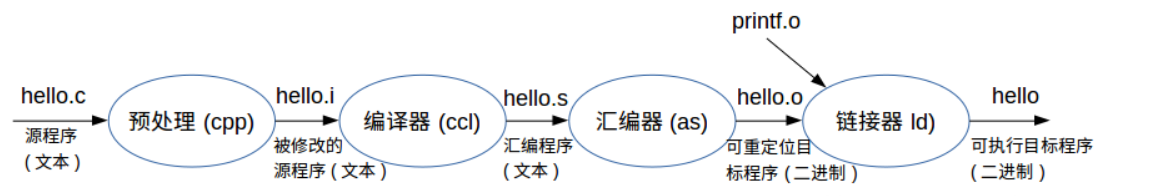
\includegraphics[width=\textwidth]{figures/02-01-C语言文件的编译流程.png}
	\caption{
		C语言文件的编译流程
	}
	\label{fig:C语言文件的编译流程}
	
	\textbf{编译NPUcore}
\end{figure}
	在shell中打开os目录后,执行make命令即可看到系统编译过程的运行截图:
	\begin{figure}[htb]
		\centering
		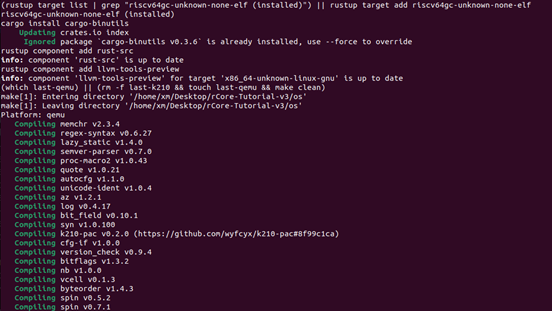
\includegraphics[width=\textwidth]{figures/02-01-NPUcore编译过程.png}
		\caption{
			NPUcore编译过程
		}
		\label{fig:NPUcore编译过程}
	\end{figure}
		\textbf{QEMU上运行NPUcore内核}
		
		在shell中输入make run即可在QEMU中启动运行NPUcore。
		QEMU相关指令如下:
		
		\begin{lstlisting}[language={Rust}, label={code:forktest},
			caption={在QEMU中启动运行NPUcore指令}]
			@qemu-system-riscv64 \
			-M 128m \
			-machine virt \
			-bios $(BOOTLOADER) \
			-device loader,file=$(KERNEL_BIN),addr=$(KERNEL_ENTRY_PA) \
			-drive file=$(FS_IMG),if=none,format=raw,id=x0 \
			-device virtio-blk-device,drive=x0 \
			-device virtio-gpu-device  \
			-device virtio-keyboard-device  \
			-device virtio-mouse-device \
			-serial stdio 
			其中:
			$(BOOTLOADER)为引导内核的BIOS的二进制文件;
			$(KERNEL_BIN)为NPUcore的二进制文件;
			$(KERNEL_ENTRY_PA)为NPUcore的二进制文件的起始执行地址;
			$(FS_IMG)为虚拟硬盘(对应现实中的硬盘);
		\end{lstlisting}
		
		运行结果图:
		
		\begin{figure}[htb]
			\centering
			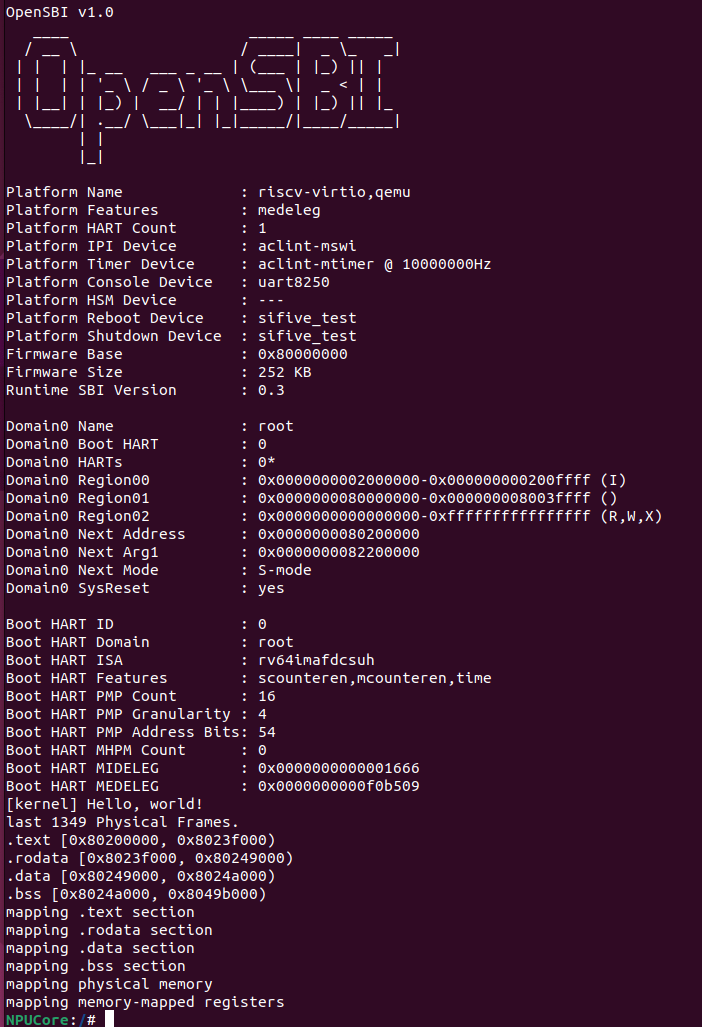
\includegraphics[width=\textwidth]{figures/02-01-NPUcore正常启动.png}
			\caption{
				NPUcore正常启动
			}
			\label{fig:NPUcore正常启动}
		\end{figure}
			在上图中,从第一行开始到“[kernel] Hello, world!”的上一行均为OpenSBI输出的相关信息,感兴趣的同学可以自行搜索SBI的相关内容,这里不做展开。
			
			\subsection{在线运行NPUcore}
			
			NPUcore操作系统内核已部署在头歌平台、Gitee、GitHub平台。为广大教师和学生学习操作系统内核构建提供线上实训支持。它也为大赛“操作系统设计赛”内核赛道区域赛顺利晋级提供支撑。可以通过在头歌平台上的实验环境在线运行NPUcore,以下是头歌平台内的链接:
			\begin{lstlisting}[language={Rust}, label={code:forktest},
				caption={NPUcore实验在头歌平台上的链接}]
				https://www.educoder.net/paths/7wnb29j6
			\end{lstlisting}
			
